%%%%%%%%%%%%%%%%%%%%%%%%%%%%%%%%%%%%%%%%%%%%
% Project Model %%%%%%%%%%%%%%%%%%%%%%%%%%%%
% Introduction to Quantum Physics Course %%%
% National Autonomous University of Mexico %%
% Created by Sergio Alfonso Pelayo Escalera %
%%%%%%%%%%%%%%%%%%%%%%%%%%%%%%%%%%%%%%%%%%%%
\documentclass[10pt]{article}
%%
\usepackage{adjustbox}
\usepackage{ulem}
\usepackage{tikz}
\usetikzlibrary{arrows.meta, positioning}
%%%
\usepackage{adjustbox}
\usepackage{array}
\usepackage{colortbl}
\usepackage{xcolor}
\usepackage{booktabs}
\usepackage{pifont} % for bullets
\definecolor{rules}{RGB}{230,235,245}
\definecolor{stats}{RGB}{230,240,230}
\definecolor{erp}{RGB}{250,235,215}

\definecolor{rulesDot}{RGB}{60,90,150}
\definecolor{statsDot}{RGB}{60,120,80}
\definecolor{erpDot}{RGB}{200,130,40}
%%%
\usepackage{tikz}
\usetikzlibrary{arrows.meta, positioning}
\usepackage{graphicx}
\usepackage{float}
\usepackage{caption}
%\citestyle{numeric}
%%
\usepackage{tikz}
\usepackage{forest}
\usepackage{pgfplots}
\usepackage{amsmath}
\pgfplotsset{compat=1.18}
\usetikzlibrary{arrows.meta, positioning, shapes.geometric}
%%
\usepackage[utf8]{inputenc}
\usepackage{fontspec}
\setmainfont{Times New Roman}
%\usepackage[T1]{fontenc}
\usepackage{tcolorbox}
\usepackage[french,english]{babel}
\usepackage{url}
\usepackage{hyperref}
\usepackage{amsmath}
\usepackage{amsfonts}
\usepackage{amssymb}
\usepackage{graphicx}
\usepackage{float}
\usepackage{lipsum}
\usepackage{multicol}
\usepackage{xcolor}
\usepackage{braket}
\usepackage{cancel}
\newcommand{\celda}[1]{
	\begin{minipage}{2.5cm}
		\vspace{5mm}
		#1
		\vspace{5mm}
	\end{minipage}
}
\definecolor{verde}{rgb}{0.24, 0.58, 0.26}
\usepackage[left=2.00cm, right=2.00cm, top=2.00cm, bottom=2.00cm]{geometry}
\author{El Argoubi El Mehdi}
\title{Explainable Anomaly Detection in Information Systems: State of the Art and Application to Timekeeping and Payroll Systems}


\usepackage{tcolorbox}
\renewenvironment{abstract}
{
  \begin{center}
  \begin{tcolorbox}[
    colback=gray!10,
    colframe=white,
    width=\textwidth,
    boxrule=0pt
  ]
  \begin{center}
  \Large\bfseries \abstractname
  \end{center}
  \par\medskip
}
{
  \end{tcolorbox}
  \end{center}
}
\makeatother
%Header Footer

\usepackage{fancyhdr}

% Disable ACM style
\pagestyle{fancy}
\fancyhf{}  % clear all header and footer fields

% Header
\fancyhead[L]{\textit{Engineering School of the Littoral Côte d’Opale}}
\fancyhead[R]{\textit{EDUREKA}}

% Footer
\fancyfoot[L]{\textit{El Argoubi El Mehdi}}
\fancyfoot[R]{\thepage}

% Optional: remove horizontal header line
\renewcommand{\headrulewidth}{0.4pt}
\renewcommand{\footrulewidth}{0.4pt}

% Link color
\hypersetup{
    colorlinks=true,
    linkcolor=blue,
    citecolor=blue,
    urlcolor=blue
}
%
\usepackage{graphicx}
\usepackage{xcolor}
\usepackage{geometry}
\usepackage{multicol}
\usepackage{tcolorbox}
\usepackage{titlesec}
\usepackage{setspace}

\geometry{margin=2cm}

\definecolor{journalblue}{RGB}{0,70,140}
\definecolor{headergray}{RGB}{220,225,230}
%%


\fancypagestyle{firstpage}{
    \fancyhf{} % empty header and footer
    \fancyfoot[L]{\textit{El Argoubi El Mehdi}}
    \fancyfoot[R]{\thepage}
    \renewcommand{\headrulewidth}{0pt}   % removes header line
    \renewcommand{\footrulewidth}{0.4pt} % keeps footer line
}


\begin{document}
\selectlanguage{english}
\thispagestyle{firstpage}

%------------------------------------------------
% HEADER JOURNAL STYLE
%------------------------------------------------

\vspace*{-1.2cm}
\noindent
\colorbox{journalblue}{%
\makebox[\dimexpr\textwidth-2\fboxsep\relax][c]{%
\parbox[c][0.25cm][c]{\textwidth}{%
\centering
\color{white}\bfseries\small
E. EL ARGOUBI / UNIVERSITY OF LITTORAL COTE D’OPALE / 2026
}}}

\vspace{0.1cm}

\noindent
\begin{minipage}{0.25\textwidth}

\includegraphics[width=1\linewidth]{eilco.png}
\end{minipage}
\hfill
\colorbox{white}{
\begin{minipage}{0.4\textwidth}
\centering
\vspace{2pt}
\vspace{2pt}
\end{minipage}
}
\hfill
\begin{minipage}{0.35\textwidth}

\includegraphics[width=1\linewidth]{Logo-ulco.png}
\end{minipage}

\vspace{0.1cm}

{\noindent\color{journalblue}\rule{\textwidth}{0.1cm}}


%------------------------------------------------
% TITLE
%------------------------------------------------
\vspace{0.4cm}

{\itshape\color{gray} \noindent \uline{Research Article}}

\vspace{0.3cm}

{
\LARGE \noindent
\textbf{EXPLAINABLE ANOMALY DETECTION IN INFORMATION SYSTEMS
STATE OF THE ART AND APPLICATION TO TIMEKEEPING AND PAYROLL SYSTEMS}\par
}


\vspace{0.5cm}

%------------------------------------------------
% AUTHORS
%------------------------------------------------

{\color{journalblue}\noindent \bfseries\scshape \Large
EL ARGOUBI El Mehdi
}
{\itshape \color{gray} \noindent \\
Engineering School of the Littoral Côte d’Opale, University of the Littoral Côte d’Opale, Calais 62100, France
}

\vspace{0.4cm}
{\color{journalblue}\hrule}
\vspace{0.4cm}

%------------------------------------------------
% ARTICLE INFO & ABSTRACT
%------------------------------------------------

\begin{minipage}[t]{0.22\textwidth}
\centering
{\color{journalblue}\textbf{A R T I C L E \quad I N F O}}

\vspace{0.1cm}
{\color{journalblue}\rule{\linewidth}{0.6pt}}
\end{minipage}
\hfill
\begin{minipage}[t]{0.73\textwidth}
{\color{journalblue}\textbf{A B S T R A C T}}

\vspace{0.1cm}
{\color{journalblue}\rule{\linewidth}{0.6pt}}
\end{minipage}

\vspace{0.5cm}

\color{black}

\begin{minipage}[t]{0.24\textwidth}
{\color{journalblue}
\textbf{Keywords:}

\vspace{0.3cm}

Information Systems\\
Fraud Detection\\
Explainable AI\\
Anomaly Detection\\
ERP\\
Human Resource Systems

\vspace{0.8cm}
}
\end{minipage}
\hfill
\begin{minipage}[t]{0.74\textwidth}
{\color{journalblue}
Timekeeping and payroll information systems play a vital role in organizations, as they process sensitive data with a direct impact on employees, regulatory compliance, and financial governance. The reliability of this data is therefore a major challenge for management processes.

However, these systems are exposed to anomalies resulting from entry errors, inconsistencies, or fraudulent behavior, which can affect data quality and user trust. Traditional control mechanisms reach their limits in the face of increasing data complexity.

In this context, the literature is moving towards automated explainable anomaly detection approaches. In sensitive areas like payroll, detection alone is insufficient and must be supplemented by explainability mechanisms.

This study proposes a state-of-the-art review of explainable anomaly detection approaches applied to timekeeping and payroll systems.
}
\end{minipage}

\vspace{0.5cm}
{\color{journalblue}\hrule}

	\vspace{3mm}
	
	\begin{multicols}{2}
		\section*{Introduction}
            Information systems are essential to the management processes of organizations, particularly timekeeping and payroll systems, which process sensitive data related to working hours and employee compensation, requiring high reliability to ensure regulatory compliance and financial governance \cite{ref1,ref2,ref3}. These systems can, however, be affected by anomalies arising from errors, inconsistencies, or abnormal behaviors, leading to malfunctions such as payment delays. In this context, traditional control mechanisms, based on fixed rules and manual verifications, reach their limits in the face of the growing complexity of data and information systems \cite{ref2}, \cite{ref3}.\\
            In this context, automatic anomaly detection appears as a promising approach to strengthen management data control mechanisms. Nevertheless, in sensitive areas such as payroll, simple identification of an anomaly is not enough. Users must be able to understand the reasons behind alerts to make informed and justifiable decisions. The explainability of anomalies is thus a central issue to strengthen user trust and ensure the auditability of automatic detection systems \cite{ref4}, \cite{ref5}.\\
            The objective of this bibliographic research is to propose a structured state of the art of explainable anomaly detection approaches in information systems, and to analyze their relevance for timekeeping and payroll systems.

            \begin{center}
            \centering
                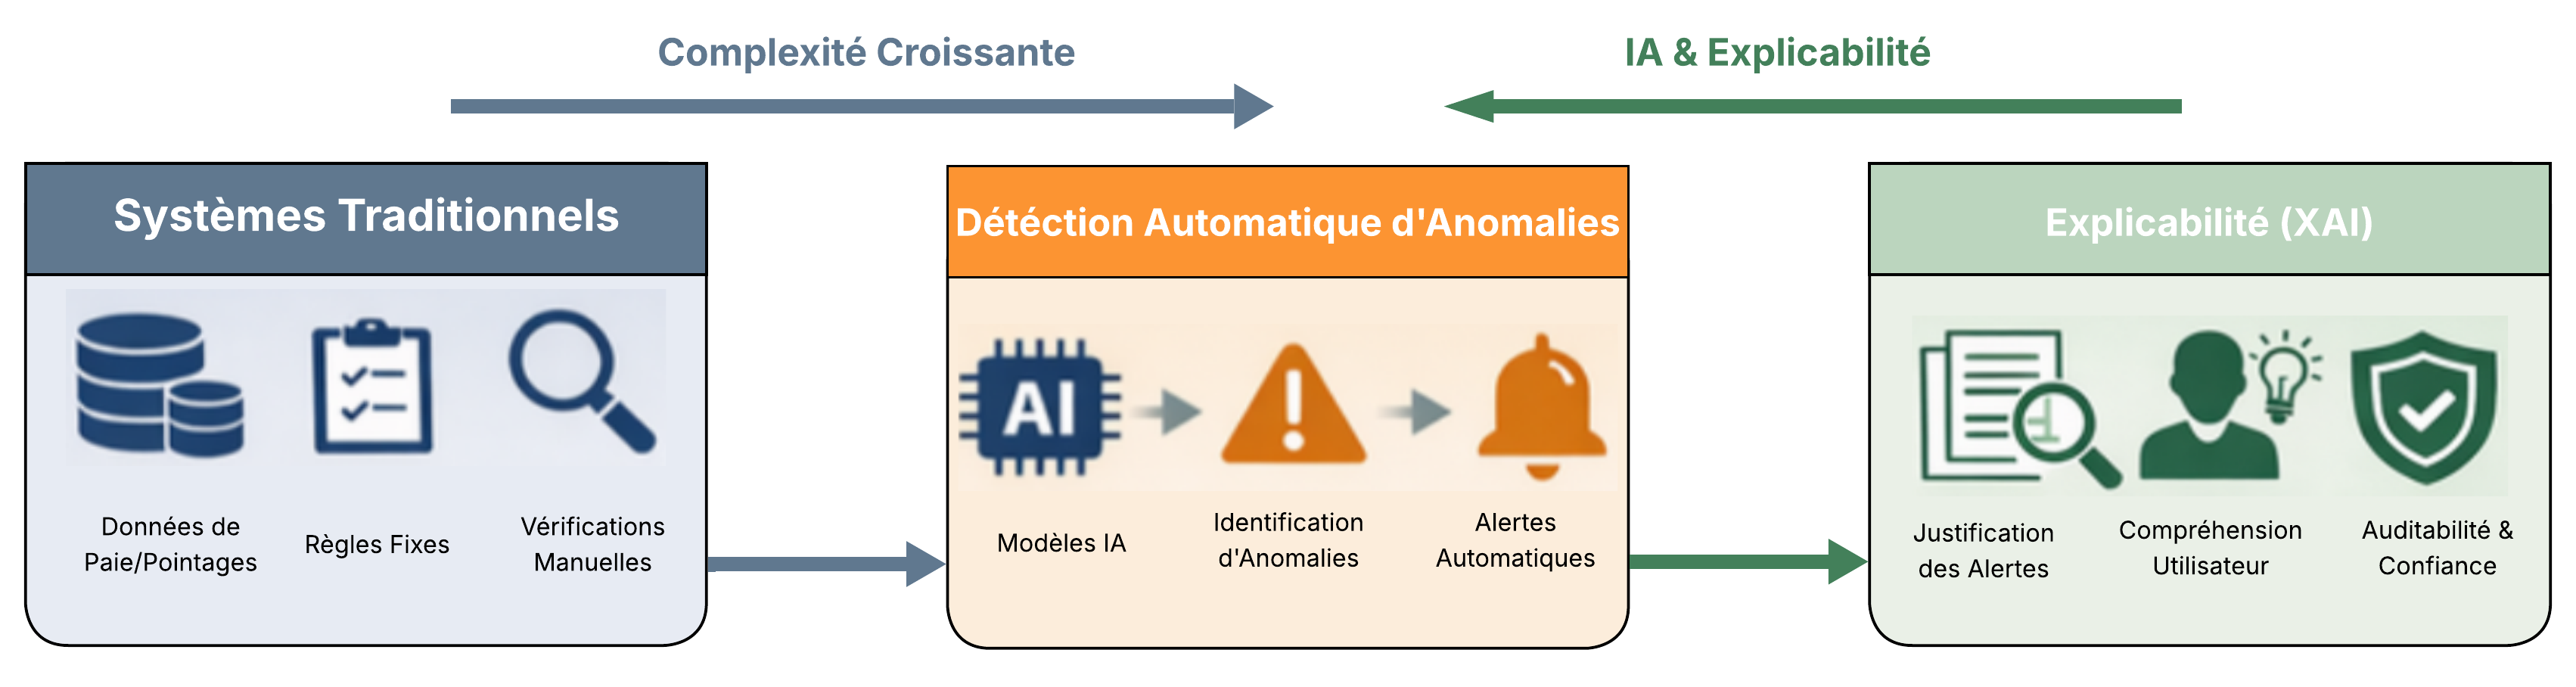
\includegraphics[width=1\linewidth]{Transition.png}
                \captionof{figure}{Transition from traditional controls to explainable anomaly detection}
            \end{center}

		\section{Anomaly detection: concepts and challenges}
            \subsection{Definition of anomalies}
            In management systems, an anomaly corresponds to a deviation from the expected operation, as defined by historical data, business rules, or organizational processes, this normality being dependent on the application context \cite{ref6}, \cite{ref7}.\\
            It is essential to distinguish anomalies from other closely related notions: errors, generally unintentional and related to data entry or processing \cite{ref8}; inconsistencies, resulting from a contradiction between information or business rules \cite{ref9}; and fraud, which involves an intentional violation of rules for gain \cite{ref2}, \cite{ref10}.\\
            An anomaly thus constitutes a generic warning signal, without assuming the cause or intention, aimed at drawing the attention of human actors to situations requiring in-depth analysis, which justifies the importance of reliable and interpretable detection mechanisms \cite{ref11}.
            \subsection{Typologies of anomalies}
            The literature distinguishes three main categories of anomalies in management systems. Statistical anomalies correspond to atypical numerical values compared to a reference behavior, frequently observed in transactional and temporal data \cite{ref8}, \cite{ref10}. Behavioral anomalies concern unusual patterns of actions or user profiles, detectable by temporal analysis or by comparison between similar entities \cite{ref12}, \cite{ref2}. Finally, logical anomalies result from violations of rules or business constraints, even when individual values appear consistent \cite{ref7}, \cite{ref9}.\\
            This typology shows that anomaly detection relies on data, behaviors, and business rules analysis, particularly in ERP systems as well as in timekeeping and payroll systems \cite{ref7}, \cite{ref6}.

            \begin{center}
            \centering
                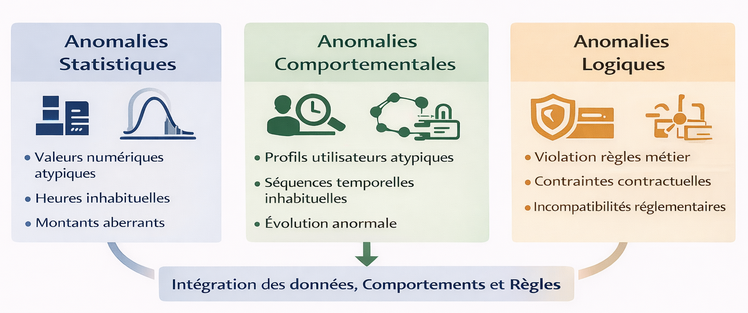
\includegraphics[width=1\linewidth]{TypologieAnomalies.png}
                \captionof{figure}{Typology of anomalies in ERP systems}
            \end{center}

        \section{Anomaly detection approaches in management systems}
        Scientific literature distinguishes several families of approaches for anomaly detection in management systems, differing by their level of automation, adaptability, and interpretation capacity. These approaches are generally grouped into three categories: rule-based approaches, statistical and exploratory approaches, and advanced approaches applied to ERP systems, where the choice strongly depends on the explainability and auditability requirements of the application context \cite{ref13}.

        \begin{center}
            \centering
            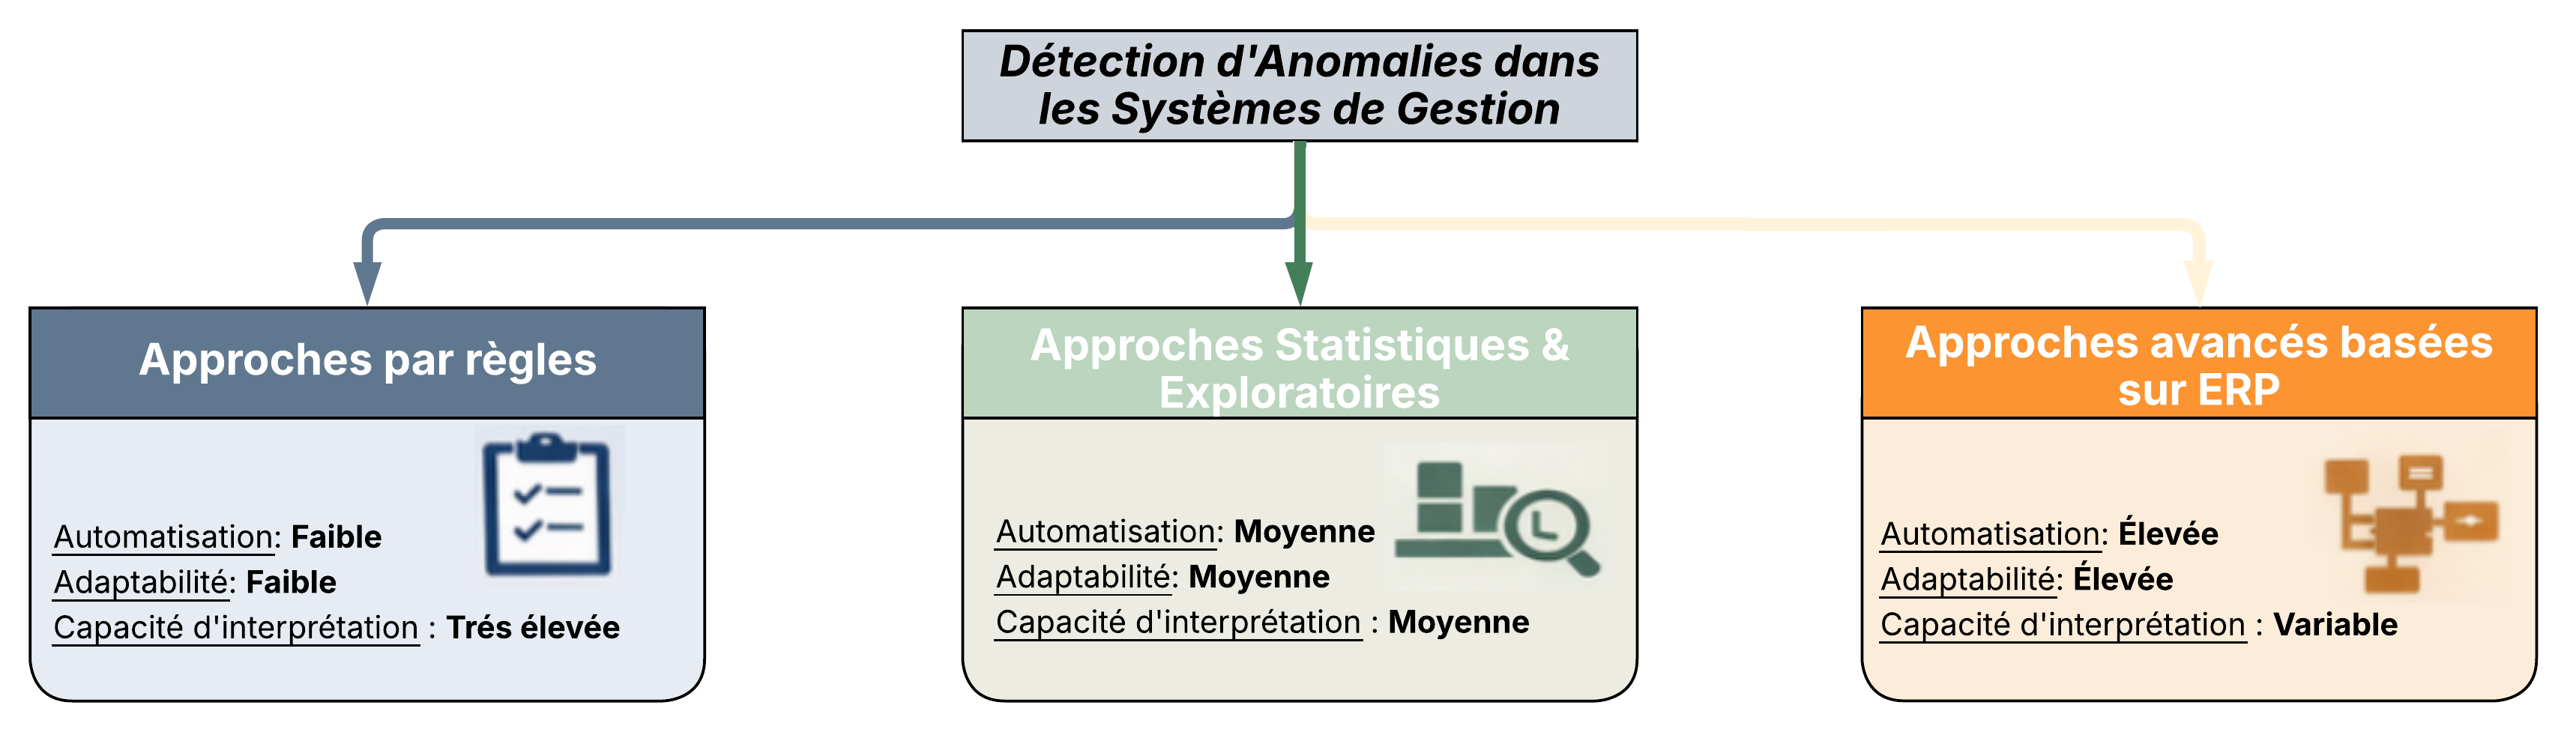
\includegraphics[width=1\linewidth]{Approches_détection.png}
            \captionof{figure}{Anomaly detection approaches in information systems}
        \end{center}
            \subsection{Rule-based approaches}
            Rule-based approaches constitute the first historical level of control in management information systems. They rely on the explicit formalization of business rules from regulatory or organizational frameworks, defining normal operating conditions for administrative and financial processes \cite{ref1}.\\
            In timekeeping and payroll systems, these rules allow verifying the consistency of declared hours and compliance of compensation calculations \cite{ref2}, \cite{ref3}. Their main advantage lies in their simplicity, transparency, and ease of audit, with rules being directly understandable by business users \cite{ref4}.\\
            However, these approaches are poorly suited to evolving behaviors, difficult to maintain at scale, and ineffective for detecting new or subtle anomalies. They can also generate a high number of false positives in complex and dynamic environments \cite{ref10}, \cite{ref13}, which motivated the development of more flexible, data-driven approaches.

            \subsection{Statistical and exploratory approaches}
            Statistical approaches detect anomalies by identifying atypical values relative to a reference behavior, based on data distribution analysis. They are particularly suited to tabular and numerical data present in management systems, notably timekeeping and payroll data \cite{ref6}.\\
            These methods allow spotting significant deviations in variables such as hours worked or compensation amounts \cite{ref8}. Profile analysis extends this approach by comparing an entity's behavior to a reference group to identify persistent anomalies \cite{ref12}.\\
            However, these approaches most often provide limited explanations, mainly indicating that a value is atypical. Some works propose associating post-hoc explanation mechanisms to specify the role of variables in the detected anomaly \cite{ref14}. Despite this, their dependence on thresholds and context-defined normality limits their robustness and interpretability in sensitive areas like payroll \cite{ref10}.

            \subsection{Advanced approaches applied to ERP}
            In ERP systems, anomaly detection increasingly relies on transactional journals and business process execution traces analysis \cite{ref7}. These approaches model event sequences, module dependencies, and user behaviors to detect process anomalies rather than simple outliers.\\
            ERP log analysis allows identifying atypical transaction sequences, process flow violations, or inconsistent user behaviors over time \cite{ref2}, \cite{ref12}. However, the complexity and heterogeneity of ERP data make anomaly interpretation difficult, requiring explainability mechanisms capable of linking detected anomalies to process steps or concerned business rules \cite{ref15}.\\
        \begin{center}
            \centering
            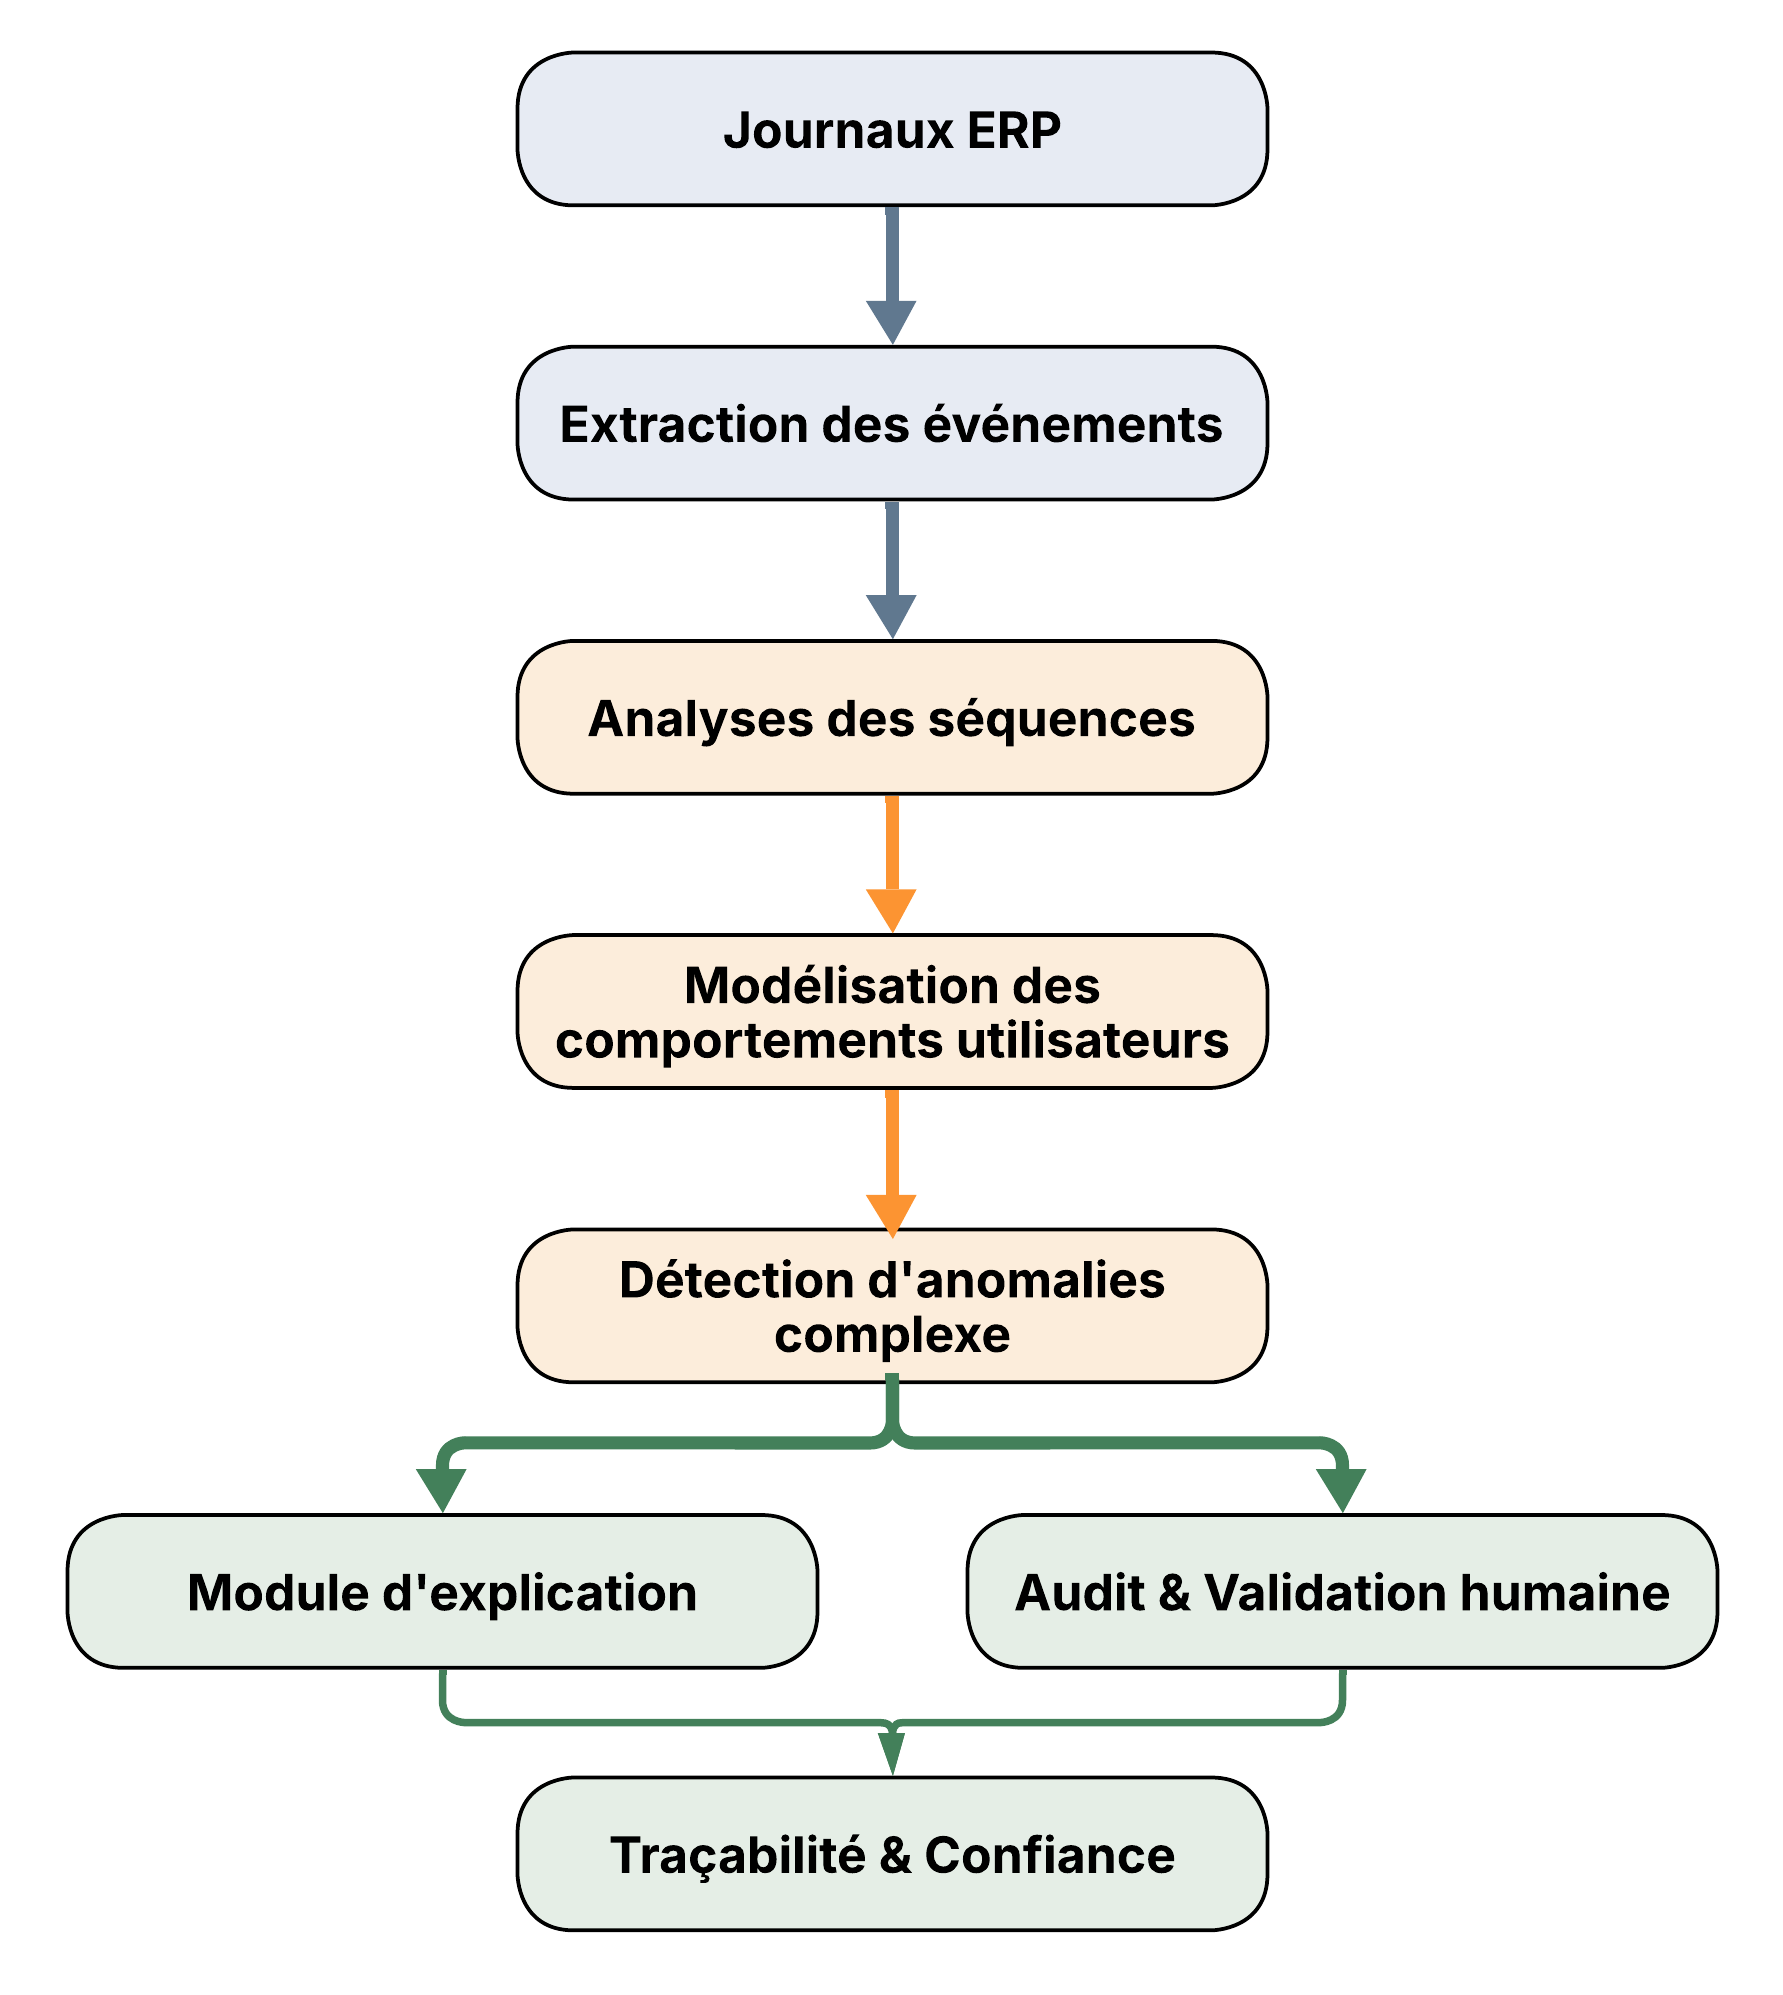
\includegraphics[width=0.9\linewidth]{journal.png}
            \captionof{figure}{Anomaly detection based on ERP log analysis}
        \end{center}

            These approaches offer better detection capacity but reinforce the need for explainable tools, particularly in payroll contexts where each anomaly must be precisely and traceably justified \cite{ref11}, \cite{ref7}, \cite{ref3}.

%%
\begin{center}

\renewcommand{\arraystretch}{1.3}
\setlength{\tabcolsep}{5pt}

\begin{adjustbox}{max width=\linewidth}
\begin{tabular}{>{\bfseries}l
                >{\columncolor{rules}}c
                >{\columncolor{stats}}c
                >{\columncolor{erp}}c}

\toprule
 & Rule-based 
 & Statistical 
 & Advanced ERP \\

\midrule
Automation & Low & Medium & High \\
Adaptability & Low & Medium & High \\
New anomaly detection & Low & Medium & High \\
Interpretability & Very high & Medium & Variable \\
Complexity & Low & Medium & High \\
Auditability & Strong & Medium & Strong if explainable \\

\bottomrule
\end{tabular}
\end{adjustbox}

\captionof{table}{Comparison of anomaly detection approaches}
\end{center}
%%
            
        \section{Explainability of anomalies}
            \subsection{Why explain an anomaly?}
            In critical management systems, an unexplained alert is hardly exploitable. Explainability transforms an automatic detection into actionable information, by identifying factors that led to the anomaly and facilitating human analysis \cite{ref4}, \cite{ref5}.\\
            Explainability also contributes to ensuring traceability and auditability of automated decisions, which is essential in sensitive areas like payroll and timekeeping \cite{ref4}. Finally, explainability promotes automatic detection systems acceptance and facilitates human validation integration in the decision-making process \cite{ref16}.

        \begin{center}

\begin{adjustbox}{max width=\linewidth}
\begin{tikzpicture}[
    node distance=0.2cm and 0.3cm,
    boxGreen/.style={
        rectangle,
        rounded corners,
        minimum width=4.2cm,
        minimum height=3.2cm,
        text width=3.8cm,
        fill=green!20,
        draw=none,
        align=center
    },
    boxBlue/.style={
        rectangle,
        rounded corners,
        minimum width=4.2cm,
        minimum height=3.2cm,
        text width=3.8cm,
        fill=blue!20,
        draw=none,
        align=center
    }
]

% Row 1
\node[boxGreen] (c) {
\textbf{Understanding}\\[8pt]
Allows explaining alerts to the user to facilitate comprehension.
};

\node[boxGreen, right=of c] (a) {
\textbf{Improvement}\\[8pt]
Helps refine models and detection rules over time.
};

% Row 2
\node[boxBlue, below=of c] (au) {
\textbf{Auditability}\\[8pt]
Facilitates alert and decision tracking for verification purposes.
};

\node[boxBlue, right=of au] (p) {
\textbf{Legal Protection}\\[8pt]
Provides legal defense in case of dispute or regulatory audit.
};

\end{tikzpicture}
\end{adjustbox}

\captionof{figure}{Benefits of explainability}
\label{fig:explainability}

\end{center}

            \subsection{Types of explanations proposed in literature}
            Literature distinguishes several families of explainability methods applied to anomaly detection. Post-hoc approaches, such as LIME and SHAP, are widely used to explain complex models, and intrinsically explainable models.\\
            LIME relies on local model approximation by building an interpretable model around the abnormal observation, allowing to identify the most locally influential variables, while SHAP relies on Shapley values theory and assigns each variable an additive contribution to the decision, offering a quantitative and consistent measure of attribute influence on detection \cite{ref4}, \cite{ref6}, \cite{ref11}.\\
            In parallel, intrinsically explainable models, such as rule-based models, logical constraints, or hybrid approaches combining symbolic logic and learning, allow integrating explainability directly into the detection process. These models explicitly link an anomaly to a business rule or constraint violation, which is particularly suited to ERP and payroll systems subject to strong regulatory requirements \cite{ref7}, \cite{ref9}.\\
            Finally, literature distinguishes between global explanations, describing general model behavior, and local explanations, centered on a specific alert. Local explanations are preferred in timekeeping and payroll systems, where each anomaly must be analyzed and validated individually \cite{ref5}, \cite{ref6}.

        \subsection{Contributions and limits of explainable approaches}
        Explainable approaches improve alert understanding, facilitate their human validation, and strengthen automated decisions traceability, which favors their integration into audit and control processes \cite{ref5}, \cite{ref11}, \cite{ref3}.\\
        However, explanation quality strongly depends on the models used and the application context. A trade-off persists between detection performance and interpretability, and objective explanation evaluation remains an open challenge \cite{ref5}, \cite{ref6}. These limits confirm that explainability remains a central research axis in management systems.

        
		\section{Application to timekeeping and payroll systems}
        Timekeeping and payroll systems rely on tabular, temporal, and highly structured data from HR and ERP systems, combining individual, contractual, and regulatory information \cite{ref1}, \cite{ref2}. This business rules dependency makes normality definition strongly contextual, while any anomaly can have financial, social, or legal consequences.\\
        In these systems, anomalies can be statistical, like an unusually high volume of hours worked, or behavioral, for example, recurrent overtime use in certain periods \cite{ref12}. Logical anomalies are particularly critical in payroll and result from explicit business rules violations, such as a conflict between overtime and work contract, a bonus allocation not provided by the collective agreement, or an inconsistency between attendance time and declared absences \cite{ref7}, \cite{ref9}.\\
        Reliability and compliance requirements mandate that these anomalies be detected before final payroll validation \cite{ref3}, \cite{ref7}. In this context, detection approaches are only truly effective if accompanied by explanation mechanisms allowing justification of alerts to business actors and control bodies \cite{ref4}, \cite{ref5}.\\
        Explainable approaches facilitate alert analysis and validation by linking anomalies to business rules, specific variables, or behavioral gaps, thus reducing investigation time \cite{ref7}, \cite{ref8}. Local explanations are particularly suited to payroll, where each alert must be examined individually \cite{ref6}, \cite{ref11}. Literature also highlights the importance of human validation to limit false positives and reinforce automated systems acceptability \cite{ref8}, \cite{ref12}, \cite{ref16}.\\
        However, works specifically dedicated to HR systems remain limited. Existing approaches are mostly transposed from other ERP contexts, without full adaptation to payroll data specificities, including their mixed, temporal, and regulated nature \cite{ref2}, \cite{ref14}, \cite{ref15}.

        \begin{center}
            \centering
            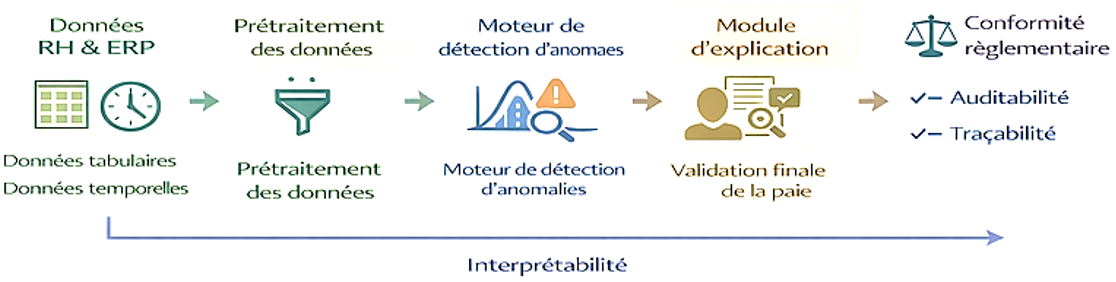
\includegraphics[width=1\linewidth]{flux.png}
            \captionof{figure}{Explainable anomaly detection approach}
        \end{center}


		\section{Discussion and research perspectives}
        Literature shows that automatic anomaly detection constitutes an important lever for management information systems control, particularly in ERP and HR environments characterized by complex and interconnected data. However, in sensitive contexts like timekeeping and payroll, detection alone is insufficient and must be supplemented by mechanisms allowing alert understanding and justification.\\
        Explainability thus appears as a central element to strengthen user trust, facilitate auditability, and support human decision-making. Nevertheless, limits persist, notably the trade-offs between detection performance and interpretability, and the difficulty of objectively evaluating explanation quality.\\
        Research perspectives mainly focus on improving explainability for mixed and temporal data, reinforced integration of business rules and human validation, as well as development of fully auditable detection frameworks compliant with critical management systems regulatory constraints.


        \section{Conclusion}
        This bibliographic research presented a state-of-the-art of explainable anomaly detection approaches in information systems, with a focus on timekeeping and payroll systems. Literature shows that traditional and statistical approaches, although useful, reach their limits facing growing complexity of data and management processes.\\
        Advanced approaches applied to ERP environments offer better detection capabilities but reinforce the need for explainability ensuring understanding, user trust, and decision auditability, particularly in sensitive contexts like payroll. Finally, research perspectives highlight the importance of adapting explainability mechanisms to mixed and temporal data, further integrating business rules and human validation, and developing fully compliant detection frameworks.


    \bigskip

    
    \bigskip
        \bibliographystyle{IEEEtran}
        \bibliography{references}

	\end{multicols}

\end{document}
